\begin{enumerate}

    \item 
    Dadas as seguintes instruções e os seus respectivos códigos de máquina,
    indique os valores dos campos OPCODE, Mod R/M, SIB, DISPLACEMENT, e IMMEDIATE.
    Note que uma instrução pode deixar de apresentar algum campo.
    \begin{itemize}
        \item [(a)] \asm{mov edx, 0x0} | ba 00 00 00 00
        \item [(b)] \asm{mov ebp, esp} | 89 e5
    \end{itemize}

    \item
    Sobre a arquitetura x64, responda:
    \begin{itemize}
        \item [(a)]
        O que significa um processador ser de arquitetura híbrida RISC/CISC?

        \item [(b)]
        Descreva como é feito o endereçamento de memória na arquitetura x64,
        indicando os grupos de bits dentro do endereçamento virtual.

        \item [(c)]
        Explique brevemente o que é a tecnologia SIMD,
        indicando os registradores envolvidos.

        \item [(d)]
        Indique as diferenças entre os registradores 
        de uso geral da arquitetura IA-32 e x64.    
    \end{itemize}

    \item
    Descreva as diferenças sobre endereçamento e utilização de memória 
    do Modo Real e o Modo Protegido. 
    Para o modo real, indique somente como é calculado o endereço de memória.
    No modo protegido, 
    faça um diagrama mostrando os diferentes segmentos de memória,
    indique como é calculado o endereço lógico e real, 
    e por que o modo é chamado de protegido.

    \item
    Uma instrução de pulo (ou salto) pode ser classificada de diversas formas.
    Responda sucintamente às perguntas abaixo com relação a pulos.
    \begin{itemize}
        \item [(a)]
        O que significa um pulo curto relativo? 
        Como é calculado o valor no contador de programa 
        após executar a instrução de pulo?

        \item [(b)]
        O que significa um pulo distante absoluto indireto?
        Como é calculado o valor no contador de programa 
        após executar a instrução de pulo?

        \item [(c)]
        Quais os tipos de pulos distantes no Protected Mode e Real Mode?
    \end{itemize}

    \item
    Os itens abaixo possuem instruções de programas Assembly IA-32 (em modo nativo) 
    que utilizam diversos modos de endereçamento. 
    Classifique cada item como correto ou errado, e justifique o que estiver errado.
    \begin{itemize}
        \item[(a)] \asm{mov eax, 10}
        \item[(b)] \asm{mov [M], al}
        \item[(c)] \asm{mov al, [cs + esi + array]}
        \item[(d)] \asm{mov vetor[1], 0}
        \item[(e)] \asm{add ax, [X + ecx]}
        \item[(f)] \asm{mov esi, vetor + ebx}
        \item[(g)] \asm{inc WORD [inicio + ebx*8 + esi]}
        \item[(h)] \asm{mov [ebx + esi*4], DWORD 5}
        \item[(i)] \asm{dec BYTE [bl]}
        \item[(j)] \asm{add [x + 1], al} 
        \item[(k)] \asm{mov eax, [array + ecx*8 + ebx]}
        \item[(l)] \asm{mov [eax*8 + 1], 5}
        \item[(m)] \asm{mov bl, ax}
        \item[(n)] \asm{cmp [esi], 10}
        \item[(o)] \asm{adc al, ah}
    \end{itemize}

    \item
    Existem três tipos básicos de operandos: imediato, registrador e memória.
    O acesso a memória pode ser feito de duas maneiras: direta ou indireta.
    Em cada instrução com algum tipo de endereçamento 
    do código abaixo especifique que tipo de operando 
    está sendo usado como fonte e destino:
    imediato, memória direta/indireta, ou registrador.
    Indicar se algum endereçamento é ilegal. 
    \putNASM{enderecamentos.asm}

    \item
    Considere o seguinte fragmento de código IA-32 obtido pelo comando \asm{objdump}.
    Como pode ser visto, a função \asm{g()} é chamada pela função \asm{f()}.
    \putC{objdump.asm}

    \begin{itemize}
        \item [(a)]
        Quantos argumentos cada uma das funções \asm{f()} e \asm{g()} recebem?
        
        \item [(b)] 
        Quando o CPU está a ponto de executar a instrução
        \asm{add} no endereço \asm{0x0804838a} em \asm{g()}, 
        mostre os valores na pilha, preenchendo a tabela abaixo.

        \begin{figure}[H]\centering
            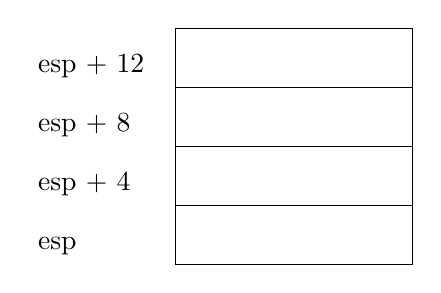
\begin{tikzpicture}[scale=.75]
                \draw
                    (0, 0) rectangle (4, 4)
                    (0, 1) --++ (4, 0)
                    (0, 2) --++ (4, 0)
                    (0, 3) --++ (4, 0)
                ;
                \draw
                  (-2.5, 3) node [above right] {\asm{esp + 12}} ++ (0, -1)
                            node [above right] {\asm{esp + 8}} ++ (0, -1)
                            node [above right] {\asm{esp + 4}} ++ (0, -1)
                            node [above right] {\asm{esp}}            
                ;
            \end{tikzpicture}
        \end{figure}
    \end{itemize}

\end{enumerate}
